\section{Query Processing and Optimization}

  \begin{definition}[Disk/Memory Blocks]
    To set up some notation, let $B(R)$ represent the number of disk blocks that relation $R$ takes up, and say $M$ is the number of blocks available in our memory. We start off with some simple operations. 
  \end{definition}

  \begin{example}[Basic Block Storage]
    Suppose we have relation $R$ with $|R| = 1000$ and each block can hold 30 tuples. Then $B(R) = \lceil 1000 / 30 \rceil = 34$, or 35 if there is overlap. 
  \end{example}

  \begin{definition}[Buffer Blocks]
    It turns out that whenever we output data to stdout, the blocks need to be stored in a \textbf{buffer block}. If the buffer block is full, then it is flushed to stdout. 
  \end{definition}

  \begin{example}[Cost of Querying Everything]
    If we do \texttt{SELECT * FROM R}, then 
    \begin{enumerate}
      \item we are at most retrieving $B(R)$ pages from disk to memory, so our IO cost is $B(R)$. 
      \item Our memory cost is 2 pages since we take each page, load it to memory, and put the answer in the output page. The next page (if any) can overwrite the previously loaded page. 
    \end{enumerate}
    We can stop early if we lookup by key. Remember that this is not counting the cost of writing the result out. 
  \end{example}

  It turns out that the efficiency of most operations defined on modern DBMS depends on two things: sorting and hashing. We'll divide up our analysis this way, focusing on their applications in joining, which tends to be the mostly used and expensive operation. Note that there are many ways to process the same query. We can in the most basic sense just scan the entire relation in disk. We can sort it. We can use a tree or hash index, and so on. All have different performance characteristics and make different assumptions about the data, so the choice is really problem-dependent. What a DBMS does is implements all alternatives and let the \textit{query optimizer} choose at runtime. We'll talk about the algorithms now and talk about the query optimizer later. 

\subsection{Brute-Force Algorithms}  

  We start off with the most brute-force algorithms of theta joins. In here, we describe how to implement it, its IO cost, and its memory cost. In the following, when we compute $R \bowtie_p S$, $R$ is called the \textbf{outer table} and $S$ the \textbf{inner table}. Furthermore, another convention is that when we calculate IO cost, we \textit{do not} factor in the cost of writing our result back to disk.  

  \subsubsection{Nested Loop Joins} 

    Our first algorithm simply takes in every block from $R$, and for every tuple $r \in R$, we take in every tuple in $S$ to calculate the predicate $p(r, s)$. 

    \begin{algo}[Nested Loop Join]
      \textbf{Nested-loop join} just uses a brute-force nested loop when computing $R \bowtie_p S$. 
      \begin{algorithm}[H]
        \caption{Nested loop Join}
        \begin{algorithmic}
          \Require{Outer table $R$, Inner table $S$}
          \Function{NestedLoop}{R, S}
            \For{each block $B_R \in R$} 
              \State load $B_R$ into memory block $M_1$
              \For{each tuple $r \in B_R$}  
                \For{each block $B_S \in S$} 
                  \State load $B_S$ into memory block $M_2$
                  \For{each tuple $s \in B_S$} 
                    \If{$p(r, s)$ is true} 
                      \State Write $r \bowtie s$ into buffer block $M_3$ 
                      \State Flush $M_3$ to stdout when it's full. 
                    \EndIf
                  \EndFor
                \EndFor
              \EndFor
            \EndFor
          \EndFunction
        \end{algorithmic}
      \end{algorithm} 
      The IO cost of this is 
      \begin{enumerate}
        \item $B(R)$ to load $R$ 
        \item For every tuple $r \in R$, we run through all of $s \in S$, requiring $B(S)$ IOs.
      \end{enumerate} 
      Therefore
      \begin{equation}
        \mathrm{IO} = B(R) + |R| \cdot B(S)
      \end{equation}
      with memory cost $3$ (since we use $M_1, M_2, M_3$ blocks).
    \end{algo}

    This is clearly not efficient since it requires a lot of IOs. We can make a slight improvement by trying to do as much as we can with the loaded blocks in memory. 

    \begin{algo}[Block-Based Nested-Loop Join]
      \textbf{Block-based nested-loop join} loops over the blocks rather than the tuples in the outer loops.  
      \begin{algorithm}[H]
        \begin{algorithmic}
          \Require{Outer table $R$, Inner table $S$}
          \Function{BlockNestedLoopJoin}{$R$, $S$}
            \For{each block $B_R \in R$} 
              \State load $B_R$ into memory block $M_1$ 
              \For{each block $B_S \in S$} 
                \State load $B_S$ into memory block $M_2$ 
                \For{each $r \in B_R, s \in B_S$} 
                  \If{$p(r, s)$ is true} 
                    \State Write $r \bowtie s$ into buffer block $M_3$ 
                    \State Flush $M_3$ to stdout when full. 
                  \EndIf 
                \EndFor
              \EndFor
            \EndFor
          \EndFunction
        \end{algorithmic}
      \end{algorithm}
      The IO cost of this is 
      \begin{enumerate}
        \item $B(R)$ to load $R$. 
        \item For every block $B_R$, we run through all of $s \in S$, requiring $B(S)$ IOs. 
      \end{enumerate}
      Therefore
      \begin{equation}
        \mathrm{IO} = B(R) + B(R) \cdot B(S)
      \end{equation}
      The memory cost is $3$ (since we use $M_1, M_2, M_3$ blocks). 
    \end{algo}

    \begin{algo}[Saturated Block-Based Nested-Loop Join]
      The next optimization is to use more memory by basically stuffing the memory with as much of $R$ as possible, stream $S$ by, and join every $S$ tuple with all $R$ tuples in memory. 
      \begin{algorithm}[H]
        \begin{algorithmic}
          \Require{Outer table $R$, Inner table $S$}
          \Function{SatBlockNestedLoopJoin}{$R$, $S$}
            \For{each set of blocks $\mathbf{B} = \{B_{i+1}, \ldots, B_{i + (M-2)}\} \subset R$} 
              \State load $\mathbf{B}$ into memory blocks $M_1, \ldots, M_{M-2}$. 
              \For{each $B_S \in S$}
                \State load $B_S$ into memory block $M_{M-1}$. 
                \For{each $r \in \mathbf{B}, s \in B_S$}  
                  \If{$p(r, s)$ is true}
                    \State Write $r \bowtie s$ into buffer block $M_M$. 
                    \State Flush $M_M$ to stdout when it's full. 
                  \EndIf
                \EndFor
              \EndFor
            \EndFor 
          \EndFunction
        \end{algorithmic}
      \end{algorithm}
      The total IO cost of this is 
      \begin{enumerate}
        \item $B(R)$ to load $R$. 
        \item For every set of $M-2$ blocks, we run through all of $s \in S$, requiring $B(S)$ IOs. 
      \end{enumerate}
      Therefore 
      \begin{equation}
        B(R) + \bigg\lceil \frac{B(R)}{M-2} \bigg\rceil \cdot B(S) \approx B(R) \cdot B(S) / M
      \end{equation}
      You want to pick the bigger table as $R$ since you want the smaller table $S$ to be loaded/streamed in multiple times. 
    \end{algo}

    \begin{algo}[Index Nested Loop Join]
      If we want to compute $R \bowtie_{R.A = S.B} S$, the idea is to use the value of $R.A$ to probe the index on $S(B)$. That is, for each block of $R$, we load it into memory, and for each $r$ in the block, we use the index on $S(B)$ to retrieve $s$ with $s.B = r.A$, and output $rs$. 

      The IO runtime, assuming that $S$ is unclustered and secondary, is 
      \begin{equation}
        B(R) + |R| \cdot (\mathrm{index lookup}) 
      \end{equation}
      Since typically the cost of an index lookup is 2-4 IOs, it beats other join methods mentioned later if $|R|$ is not too big. Since this does not scale at all with $S$, it is better to pick $R$ to be the smaller relation. The memory requirement as with other operations is $3$ blocks. 
    \end{algo}

\subsection{Sort-Based Algorithms}

  \subsubsection{External Merge Sort}

    Now let's talk about processing of queries, namely how sorting works in a database system, called \textbf{external merge sort}. In an algorithm course, we know that the runtime is $O(n \log{n})$, but this is for CPU comparisons where the entire list is loaded in memory. This is extremely trivial in comparison to the IO commands we use in databases, so we will compute the runtime of sorting a relation by an attribute in terms of IO executions. 

    The problem is that we want to sort $R$ but $R$ does not fit in memory. We divide this algorithm into \textbf{passes} which deals with intermediate sequences of sorted blocks called \textbf{runs}. 
    \begin{enumerate}
      \item Pass 0: Read $M$ blocks of $R$ at a time, sort them in memory, and write out the sorted blocks, which are called \textit{level-0 runs}. 
      \item Pass 1: Read $M-1$ blocks of the level $0$ runs at a time, sort/merge them in memory, and write out the sorted blocks, which are called \textit{level-1 runs}.\footnote{The reason we need $M-1$ rather than $M$ is that now we are merging. We are not merging in-place so we need this extra buffer to store as we traverse our pointers down each of the $M-1$ blocks.}
      \item Pass 2: Read $M-1$ blocks of the level $1$ runs at a time, sort/merge them in memory, and write out the sorted blocks, which are called \textit{level-2 runs}. 
      \item ...  
      \item Final pass produces one sorted run. 
    \end{enumerate}

    \begin{figure}[H]
      \centering 
      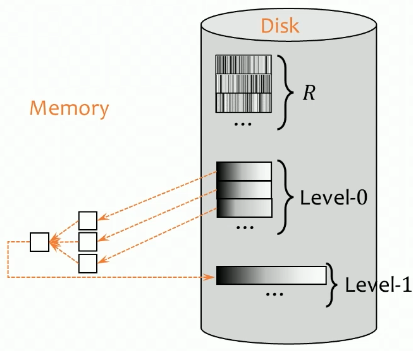
\includegraphics[scale=0.4]{img/merge.png}
      \caption{} 
      \label{fig:merge}
    \end{figure}

    \begin{algo}[External Merge Sort]
      The implementation has a lot of details. Not finished yet. 
      \begin{algorithm}[H]
        \begin{algorithmic}
          \Require{Relation $R$}
          \Function{ExternalMergeSort}{$R$} 
            \State $L = [0]$ \Comment{Array storing number of level-$i$ runs}
            \While{while there are blocks to read from $R$} \Comment{First pass}
              \State read the next $M$ blocks $B = \{B_1, \ldots, B_M \}$ at a time and store it in memory.
              \State sort $B$ to generate a level-0 run $B^{(0)} = \{B_1^\prime, \ldots, B_M^\prime \}$.
              \State write $B^{(0)}$ to disk. 
              \State $L[0] += 1$
            \EndWhile

            \While{$L[-1] \geq M$} 
              \State append $0$ to $L$ 
              \State let $\mathbf{B} = \{B\}$ be the set of previous runs 
              \While{there exists blocks to be read in $\mathbf{B}$} 
                \State read $M-1$ blocks starting from the beginning of each run into memory. 
                \State sort them to produce the $i$th run $B^{(i)}$. 
                \State write $B^{(i)}$ to disk. 
              \EndWhile
            \EndWhile

          \EndFunction
        \end{algorithmic}
      \end{algorithm}
      To compute the cost, we know that 
      \begin{enumerate}
        \item in pass 0, we read $M$ blocks of $R$ at a time, sort them, and write out a level 0 run, so there are 
          \begin{equation}
            \lceil B(R) / M \rceil
          \end{equation}
          level 0 sorted runs, or passes. 

        \item in pass $i$, we merge $M-1$ level $(i-1)$ runs at a time, and write out a level $i$ run. We have $M-1$ memory blocks for input and $1$ to buffer output, so 
          \begin{equation}
            \text{Num. of level i runs} = \bigg\lceil \frac{\text{Num. of level (i-1) runs}}{M-1} \bigg\rceil 
          \end{equation}

        \item The final pass produces 1 sorted run. 
      \end{enumerate}

      Therefore, the number of passes is approximately 
      \begin{equation}
        \bigg\lceil \log_{M-1} \Big\lceil \frac{B(R)}{M} \Big\rceil \bigg\rceil + 1
      \end{equation}
      and the number of IOs is $2 B(R)$ since each pass reads the entire relation once and write it once. The memory requirement is $M$ (as much as possible). 
    \end{algo}

    \begin{example}[Baby Merge]
      Assume $M = 3$, with each block able to hold at most 1 number. Assume that we have an input (relation) 
      \begin{equation}
        1, 7, 4, 5, 2, 8, 3, 6, 9
      \end{equation}
      Then we go through multiple passes. 
      \begin{enumerate}
        \item Pass 0 will consist of 3 runs. You load each of the 3 numbers in memory and sort them.  
          \begin{align}
            1, 7, 4 & \mapsto 1, 4, 7 \\ 
            5, 2, 8 & \mapsto 2, 5, 8 \\ 
            9, 6, 3 & \mapsto 3, 6, 9
          \end{align}

        \item Pass 1. You merge them together by first taking 1 and 2, loading them in memory, and then comparing which one should go first. Once 1 is outputted, then the next number 4 overwrites 1 in memory, and then 2 is outputted, and so on. 
          \begin{align}
            & 1, 4, 7 + 2, 5, 8 \mapsto 1, 2, 4, 5, 7, 8 \\ 
            & 3, 6, 9
          \end{align}

        \item Pass 2. Merges the final two relations. 
          \begin{align}
            1, 2, 3, 4, 5, 7, 8 + 3, 6, 9 \mapsto 1, 2, 3, 4, 5, 6, 7, 8, 9
          \end{align}
      \end{enumerate}
      Therefore, pass 0 uses all $M$ pages to sort, and after that, when we merge, we only use $M-1$ pages to merge the inputs together and $1$ page for the output. 
    \end{example}

    Some performance improvements include: 
    \begin{enumerate}
      \item \textit{Double Buffering}. You allocate an additional block for each run, and while you are processing (merging the relations in memory), you run the IO concurrently and store it in the new block to save some time. 
      \item \textit{Blocked IO}. Instead of reading/writing one disk block at a time, we can read/write a bunch of them in clusters. This is sort of like parallelization where you don't output just one block, but multiple blocks done from multiple processing. 
    \end{enumerate}
    The problem with both of these is that we have smaller fan-in, i.e. more passes. Since we are using more blocks per run than we have, we can look at fewer runs at once. 

  \subsubsection{Sort Merge Joins}

    Now that we know how to sort, let's exploit this to optimize joins beyond nested-loops. We introduce a naive version of sort-merge join. 

    \begin{algo}[Naive Sort-Merge Join]
      A clever way is to first sort $R$ and $S$ by their join attributes, and then merge. Given that the first tuples in sorted $R, S$ is $r, s$, we do repeat until one of the $R$ or $S$ is exhausted. 
      \begin{enumerate}
        \item If $r.A > s.B$, then $s =$ next tuple in $S$ 
        \item Else if $r.A < s.B$, then $r =$ next tuple in $R$. 
        \item Else output all matching tuples and $r, s$ = next in $R, S$, which is basically a nested loop. 
      \end{enumerate}
      Therefore, given that it takes $\mathrm{sort}(R), \mathrm{sort}(S)$ to sort $R, S$ (the equations above is too cluttered to write), the IO cost consists of
      \begin{enumerate}
        \item Sorting $R$ and $S$. 
        \item We then must write $R$ and $S$ to disk in order to prepare for merging, so $B(R) + B(S)$. 
        \item We then must write $R$ and $S$ back into memory, one at a time, to merge them, so $B(R) + B(S)$. 
      \end{enumerate}
      Therefore, the IO is really just $2 B(R) + 2 B(S)$ more than it takes to sort both $R$ and $S$. 
      \begin{equation}
        \mathrm{IO} = \mathrm{sort}(R) + \mathrm{sort}(S) + 2 B(R) + 2 B(S)
      \end{equation}
      which is worst case $B(R) \cdot B(S)$ when everything joins. 
      \begin{algorithm}[H]
        \caption{}
        \label{alg:}
        \begin{algorithmic}
          \Require{}
          \State 
          \Function{Func}{x}
          \EndFunction
        \end{algorithmic}
      \end{algorithm}
    \end{algo}

    \begin{example}[Worst Case]
      To see the worst case when the IO cost is $B(R) \cdot B(S)$, look at the following example. By the time we got to the first $3$, we can't just increment the pointers for both relations. We must scan through all of the tuples of A with value 3 and all those in B with value 3 and do a nested loop to join them. 
      
      \begin{figure}[H]
        \centering 
        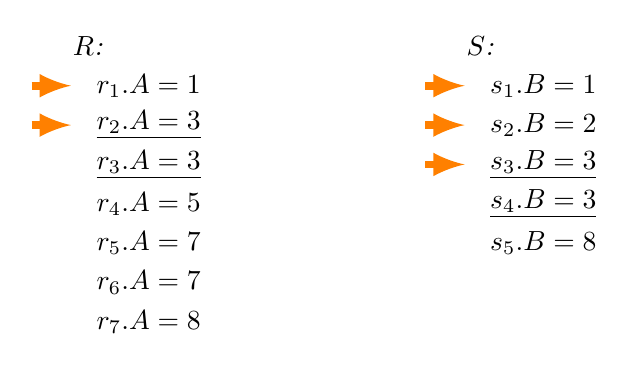
\begin{tikzpicture}[
          every node/.style={font=\normalfont}
          ]
          
          % Headers
          \node[font=\itshape, anchor=west] at (0.2,3.5) {$R$:};
          \node[font=\itshape, anchor=west] at (5.2,3.5) {$S$:};
          
          % R equations
          \node[anchor=west] at (0.5,3) {$r_1.A = 1$};
          \node[anchor=west] at (0.5,2.5) {$\underline{r_2.A = 3}$};
          \node[anchor=west] at (0.5,2) {$\underline{r_3.A = 3}$};
          \node[anchor=west] at (0.5,1.5) {$r_4.A = 5$};
          \node[anchor=west] at (0.5,1) {$r_5.A = 7$};
          \node[anchor=west] at (0.5,0.5) {$r_6.A = 7$};
          \node[anchor=west] at (0.5,0) {$r_7.A = 8$};
          
          % S equations
          \node[anchor=west] at (5.5,3) {$s_1.B = 1$};
          \node[anchor=west] at (5.5,2.5) {$s_2.B = 2$};
          \node[anchor=west] at (5.5,2) {$\underline{s_3.B = 3}$};
          \node[anchor=west] at (5.5,1.5) {$\underline{s_4.B = 3}$};
          \node[anchor=west] at (5.5,1) {$s_5.B = 8$};
          
          % Orange arrows for highlighted elements - completely straight
          \draw[orange, line width=1mm, -latex] (-0.2,3) -- (0.3,3);
          \draw[orange, line width=1mm, -latex] (-0.2,2.5) -- (0.3,2.5);
          \draw[orange, line width=1mm, -latex] (4.8,3) -- (5.3,3);
          \draw[orange, line width=1mm, -latex] (4.8,2.5) -- (5.3,2.5);
          \draw[orange, line width=1mm, -latex] (4.8,2) -- (5.3,2);
          
        \end{tikzpicture}
        \caption{Before you increment the next pointer, you must loop through all combinations of the underlined elements in the left and right relations.}
        \label{fig:nested_loop}
      \end{figure}
    \end{example}

    We have completely isolated the sorting phase and the merging phase, but we don't have to do this. Just like regular merge-sort, we can integrate them together to save IO in the last merge phase. 

    \begin{algo}[Optimized Sort-Merge Join] 
      The algorithm is just slightly modified from the naive implementation. After the final pass from sorting both $R$ and $S$, say that we have $W_R$ and $W_S$ final runs such that 
      \begin{equation}
        M > W_R + W_S
      \end{equation} 
      We can assume that this is true since if it wasn't, we can just add another pass of external sort to reduce one of the $W$'s. Then, we can do these 3 things simultaneously. 
      \begin{enumerate}
        \item We can load in the next smallest block from $R$ from its runs, merge them together.
        \item We can load in the next smallest block from $S$ form its runs, merge them together. 
        \item We can join the merged blocks \textit{in memory} and output to the buffer to be flushed. 
      \end{enumerate}

      This saves us the IO cost of writing the sorted runs back into memory and then loading them again to write, giving us a total IO cost that is equal to that of simply sorting $R$ and $S$. 
      \begin{equation}
        \mathrm{IO} = \mathrm{sort}(R) + \mathrm{sort}(S)
      \end{equation} 
      The memory varies depending on how many passes, but if $R$ and $S$ are moderately big in that we need full memory to sort them, then the memory cost is $M$ (we use everything). 

      \begin{figure}[H]
        \centering 
        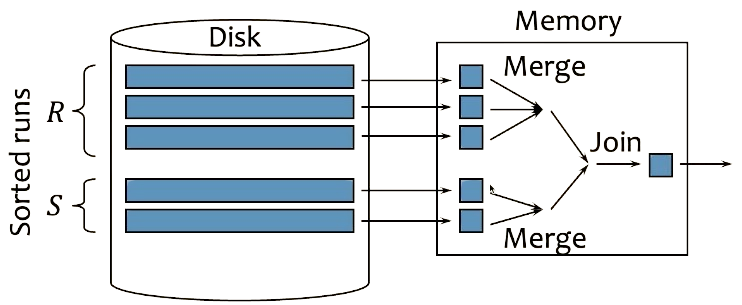
\includegraphics[scale=0.4]{img/smj_optim.png}
        \caption{Sorting: produce sorted runs for $R$ and $S$ such that there are fewer than $M$ of them total. Then in merge and join, we merge the runs of $R$, merge the runs of $S$, and merge-join the result streams as they are generated!} 
        \label{fig:smj_optim}
      \end{figure}
    \end{algo}

    \begin{example}[Two-Pass SMJ] 
      If SMJ completes in two passes, then the IOs is really cheap since we are basically getting a $2 B(R) + 2 B(S)$ cost of a level-0 pass, plus the final merge-join step which takes another $B(R) + B(S)$. 
      \begin{equation}
        \mathrm{IO} = 3 ( B(R) + B(S)) 
      \end{equation}
      If SMJ cannot complete in 2 passes, then we repeatedly merge to reduce the number of runs as necessary before the final merge and join. 
    \end{example}

  \subsubsection{Zig-Zag Join} 

    \begin{definition}[Zig Zag Join using Ordered Indices]
      To compute $R \bowtie_{R.A = S.B} S$, the idea is to use the ordering provided by the indices on $R(A)$ and $S(B)$ to eliminate the sorting step of merge-join. The idea is similar to sort-merge join. We start at the leftmost leaf node of both indices of $R$ and $S$, and traverse (right) through the leaves, querying both of the data at leaf $a$ in $R$ and $b$ in $S$ if the leaf values are equal. 

      Note that we don't even have to traverse through all leaves. If we find that a key is large, we can just start from the root node to traverse, possibly skipping many keys that don't match and not incurring all those IO costs. This can be helpful if the matching keys are distributed sparsely.

      \begin{figure}[H]
        \centering 
        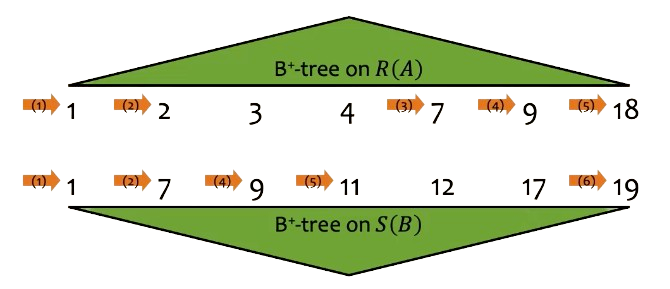
\includegraphics[scale=0.4]{img/zig_zag.png}
        \caption{We see that the B+ tree of $B$ has value $7$ while that of $A$ has value $2$. Rather than traversing $2 \mapsto 3 \mapsto 4 \mapsto 7$, we can just traverse to $7$ from the root node of $A$. This can give us a stronger bound. } 
        \label{fig:zig_zag}
      \end{figure}
    \end{definition}

  \subsubsection{Other Sort Based Algorithms}

    The set union, intersection, difference is pretty much just like SMJ. 

    For duplicate elimination, you simply modify it so that during both the sort and merge steps, you eliminate duplicates if you find any. 

    For grouping and aggregation, you do external merge sort by the group-by columns. The trick is you produce ``partial'' aggregate values in each run and combine them using merge. 

\subsection{Hash-Based Algorithms}

  \subsubsection{Hash Join} 

    Hash joining is useful when dealing with equality predicates: $R \bowtie_{R.A = S.B} S$. 

    \begin{definition}[Hash Join]
      The main idea of \textbf{hash join} is that we want to partition $R$ and $S$ by hashing (using a hash function that maps to $M-1$ values) their join attributes and then consider corresponding partitions (that get mapped to the same hash value) of $R$ and $S$. If $r.A$ and $s.B$ get hashed to the same number, they might join, and if they don't, then they definitely won't join. The figure below nicely visualizes this. 

      \begin{figure}[H]
        \centering 
        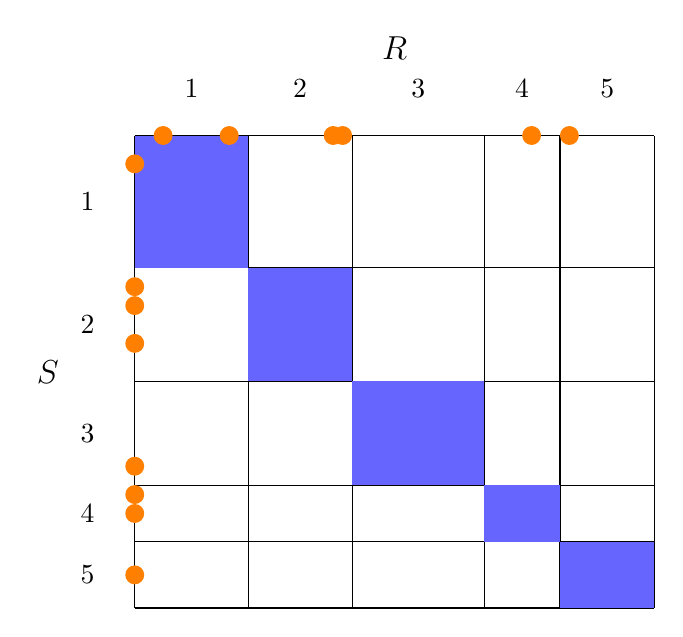
\begin{tikzpicture}[
            scale=1.2,
            every node/.style={font=\normalfont}
          ]
          
          % Grid with uneven spacing
          % Vertical lines
          \draw (0,0) -- (0,5);
          \draw (1.2,0) -- (1.2,5);
          \draw (2.3,0) -- (2.3,5);
          \draw (3.7,0) -- (3.7,5);
          \draw (4.5,0) -- (4.5,5);
          \draw (5.5,0) -- (5.5,5);
          
          % Horizontal lines
          \draw (0,0) -- (5.5,0);
          \draw (0,0.7) -- (5.5,0.7); 
          \draw (0,1.3) -- (5.5,1.3);
          \draw (0,2.4) -- (5.5,2.4);
          \draw (0,3.6) -- (5.5,3.6);
          \draw (0,5) -- (5.5,5);
          
          % Fill diagonal cells with blue
          \fill[blue!60] (0,3.6) rectangle (1.2,5);
          \fill[blue!60] (1.2,2.4) rectangle (2.3,3.6);
          \fill[blue!60] (2.3,1.3) rectangle (3.7,2.4);
          \fill[blue!60] (3.7,0.7) rectangle (4.5,1.3);
          \fill[blue!60] (4.5,0) rectangle (5.5,0.7);
          
          % Row labels (S)
          \node at (-0.5,4.3) {1};
          \node at (-0.5,3.0) {2};
          \node at (-0.5,1.85) {3};
          \node at (-0.5,1.0) {4};
          \node at (-0.5,0.35) {5};
          \node[font=\large, anchor=east] at (-0.7,2.5) {$S$};
          
          % Column labels (R)
          \node at (0.6,5.5) {1};
          \node at (1.75,5.5) {2};
          \node at (3.0,5.5) {3};
          \node at (4.1,5.5) {4};
          \node at (5.0,5.5) {5};
          \node[font=\large, anchor=south] at (2.75,5.7) {$R$};
          
          % Random orange dots along top edge (6 dots)
          \fill[orange] (0.3,5) circle (0.1);
          \fill[orange] (1.0,5) circle (0.1);
          \fill[orange] (2.1,5) circle (0.1);
          \fill[orange] (2.2,5) circle (0.1);
          \fill[orange] (4.2,5) circle (0.1);
          \fill[orange] (4.6,5) circle (0.1);
          
          % Random orange dots along left edge (8 dots)
          \fill[orange] (0,0.35) circle (0.1);
          \fill[orange] (0,1.0) circle (0.1);
          \fill[orange] (0,1.5) circle (0.1);
          \fill[orange] (0,1.2) circle (0.1);
          \fill[orange] (0,2.8) circle (0.1);
          \fill[orange] (0,3.4) circle (0.1);
          \fill[orange] (0,3.2) circle (0.1);
          \fill[orange] (0,4.7) circle (0.1);
          
        \end{tikzpicture}
        \caption{Say that the orange points represent the hashed values of $r.A$ and $s.B$ for $r, s \in R, S$. The nested loop considers all slots (all pairs of orange points between $R$ and $S$), but hash join considers only those along the diagonal. } 
        \label{fig:hash_join}
      \end{figure}

      Then, in the \textbf{probing phase}, we simply read in each partition (the set of tuples that map to the same hash) of $R$ into memory, stream in the corresponding partition of $S$, compare their \textit{values} (not hashes since they are equal), and join if they are equal. If we cannot fit in a partition into memory, we just take a second hash function and hash it again to divide it into even smaller partitions (parallels merge-sort join). 

      \begin{figure}[H]
        \centering 
        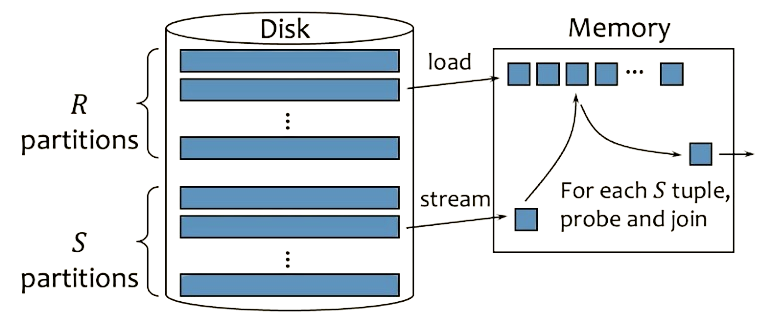
\includegraphics[scale=0.4]{img/hash_join2.png}
        \caption{} 
        \label{fig:hash_join2}
      \end{figure}

      Therefore, if the hash join completes in two passes, the IO runtime is 
      \begin{equation}
        3 ( B(R) + B(S)) 
      \end{equation}
      which is similar to merge-sort join. As for the memory requirement, let's first assume that in the probing phase, we should have enough memory to fit one partition of $R$, i.e. $M-1 > \lceil B(R) / (M-1) \rceil$, so solving for it roughly gives $M > \sqrt{B(R)} + 1$. We can always pick $R$ to be the smaller relation, so roughly 
      \begin{equation}
        M > \sqrt{\min\{ B(R), B(S)\}} + 1
      \end{equation}
    \end{definition}

    \begin{theorem}[Hash vs Sort-Merge Join]
      To compare hash join and SMU, note that their IOs are the same, but for memory requirements, hash join is lower, especially when the two relations have very different sizes. 
      \begin{equation}
        \sqrt{\min\{B(R), B(S)\}} + 1 < \sqrt{B(R) + B(S)}
      \end{equation}
      Some other factors include the quality of the hash (may not generate evenly sized partitions). Furthermore, hash join does not support inequality joins unlike SMJ, and SMJ wins if either $R$ and/or $S$ is already sorted. SMJ also wins if the result needs to be in sorted order. 
    \end{theorem}

    Sometimes, even block nested loop join may win in the following cases. 
    \begin{enumerate}
      \item if many tuples join (as in the size of the join is $|S| \cdot |R|$) since we are doing unnecessary processing in hash/merge-sort joins. 
      \item if we have black-box predicates where we may not know the truth/false values of the $\theta$
    \end{enumerate}

  \subsubsection{Other Hash Based Algorithms}

    The union, difference, and intersection are more or less like hash join. 

    For duplicate elimination, we can check for duplicates within each partition/bucket. 

    For grouping/aggregation, we can apply the hash functions to the group-by columns. Tuples in the same group must end up in the same partition/bucket. Or we may keep a running aggregate value for each group. 

    To compare the duality of sort and hash, note that 
    \begin{enumerate}
      \item in sorting, we have a physical division and logical combination 
      \item in hashing, we have a logical division and physical combination
    \end{enumerate}
    When handling large inputs, 
    \begin{enumerate}
      \item in sorting we have multi-level merge 
      \item in hashing we have recursive partitioning 
    \end{enumerate}
    For IO patterns, 
    \begin{enumerate}
      \item in sorting we have sequential write and random read (merge) 
      \item in hashing we have random write and sequential read (partition) 
    \end{enumerate}

\subsection{Exercises} 

  Here are some exercises for calculating IO costs of these joins. 

  \begin{example}[Join Operations]
    Consider the two tables
    \begin{enumerate}
      \item \texttt{Orders(OrderID, CustomerID, OrderDate, TotalAmount)} 
      \item \texttt{Customers(CustomerID, Address)}
    \end{enumerate}
    \texttt{Orders.CustomerID} is a foreign key referring to \texttt{Customers.CustomerID}.

    The rows are not sorted on any particular attribute. We want to join the two tables using the attribute CustomerID:
    \[
    \text{Orders} \bowtie_{\text{Orders.CustomerID = Customers.CustomerID}} \text{Customers}
    \]
    The inner and outer tables can be swapped to reduce I/O costs in the following questions.

    Assume the following:
    \begin{itemize}
      \item The cost metric is the number of page/block I/Os unless otherwise noted.
      \item DO NOT count the I/O cost of writing out the final result unless otherwise noted.
      \item M = 19 blocks (= pages) available in memory unless otherwise noted.
      \item Table Orders contains 50,000 records (rows/tuples) on disk. One block can contain 20 Orders-tuples.
      \item Table Customers contains 20,000 records (rows/tuples) on disk. One block can contain 10 Customers-tuples.
      \item Assume uniform distribution for Orders.CustomerID and Customers.CustomerID -- i.e. the same number of Orders-tuples join with a Customers-tuple.
      \item Ignore page boundary wherever applicable.
      \item Assume uniform distributions wherever applicable.
    \end{itemize}

    \vspace{1em}
    \noindent\textbf{Question 2.1}
    \begin{enumerate}[label=(\alph*)]
      \item For the Orders and Customers tables, we want to perform a nested-loop join (\textbf{using 3 memory blocks}). What is the \textbf{minimum} total I/O cost? (Choose the table that will reduce the I/O cost as the outer table.)
      
      \item For the Orders and Customers tables, we want to perform a block-based nested-loop join (\textbf{using 3 memory blocks}). What is the \textbf{minimum} total I/O cost?
    \end{enumerate}

    For (a), we choose $R = $ Customers as the outer table since it is smaller. Therefore, our IO cost is 
    \begin{equation}
      B(R) + |R| \cdot B(S)  = 2000 + 20,000 \cdot 2500 = 50,002,000
    \end{equation}

    For (b), we also choose $R = $ Customers as outer since it's smaller. The IO cost is 
    \begin{equation}
      B(R) + B(R) \cdot B(S)= 2000 + 2000 * 2500 = 5,002,000
    \end{equation}

    \vspace{1em}
    \noindent\textbf{Question 2.2}
    \begin{enumerate}[label=(\alph*)]
      \item If we want to perform an external merge sort on the Orders table, how many level-0 runs does the external merge sort produce for the Orders table (M=19)?
      
      \item Continuing with the question (a), how many passes in total does the external merge sort take (including the first sorting pass)? Show the calculations for each pass (including the number of runs and size of each run).
      
      \item What is the total I/O cost of the external merge sort for the Orders table? Remember, do not count the cost of final write.
      
      \item Do an improved sort-merge-join, i.e., do merge and join in the same pass when the total number of sorted runs from Orders and Customers will fit in memory including an output block. Compute the minimum total I/O cost of sort-merge-join of table Orders and Customers.
    \end{enumerate}

    For (a), we read $M$ blocks of $R$ at a time, so we need to have $\lceil B(R) / M \rceil = \lceil 2500 / 19 \rceil =$ \textbf{132 passes}. 

    For (b), we saw that 
    \begin{enumerate}
      \item The level 0 pass takes 132 runs. 
      \item The level 1 pass takes $\lceil 132 / (19 - 1) \rceil = 8$ runs. 
      \item At this point we can just run once more since $8 < 18$, so our level 2 pass takes $1$ run. 
    \end{enumerate}
    So we have \textbf{3 passes} with \textbf{141 runs}. 

    For (c), we have $B(R) = 2500$ and just compute the following. 
    \begin{enumerate}
      \item For level $0$, we read all blocks, and write them all out: $2 B(R)$. 
      \item For level 1, it's the same thing since we again read all blocks and write them back to disk: $2 B(R)$. 
      \item For level 2, we just read through and do not include the final write, so $B(R)$.
    \end{enumerate}
    This is a total of \textbf{$5 B(R) = 5 \cdot 2500 =$ 12,500 IOs}. 

    For (d), 
    \begin{enumerate}
      \item For the first pass, you load all blocks of both relations in memory for the first iteration of sort merge and then write them to disk, giving us $2 (B(R) + B(S))$ IOs. 
      \item The second pass is the same, giving us $2 (B(R) + B(S))$ IOs. 
      \item By the third pass, we complete the sort-merge join giving us $B(R) + B(S)$. 
    \end{enumerate}
    This is a total of $5 (B(R) + B(S)) = 5 \cdot (2000 + 2500) =$ \textbf{22,500 IOs}. 

    \vspace{1em}
    \noindent\textbf{Question 2.3}
    Assume uniform distribution for the hash function(s).
    \begin{enumerate}[label=(\alph*)]
        \item For the Orders and Customers tables, we want to perform a multi-pass hash join. How many passes do we need (including partitioning phase and join phase)?
        
        \item What is the minimum I/O cost of joining Orders and Customers using a hash join?
        
        \item What is the minimum number of memory blocks required if we want to perform a 2-pass hash join? Note that M should be an integer.
    \end{enumerate}

    For (a), we must partition both relations. 
    \begin{enumerate}
      \item In the first partition pass, we 
        \begin{enumerate}
          \item take Customers and have $\lceil 2000 / (19 - 1) \rceil = 112 > 18$. Each partition contains 112 blocks, which is too big for our memory, so we must partition again.
          \item take Orders and have $\lceil 2500 / (19 - 1) \rceil = 139$. Each partition contains 139 blocks, which is too big for our memory, so we must partition again.
        \end{enumerate}
      \item In the second partition pass, we 
        \begin{enumerate}
          \item take Customers and have $\lceil 112 / 18 \rceil = 7 \leq 18$, so we are done since each partition (of a partition) of 7 blocks can fit in memory.  
          \item take Orders and have $\lceil 139 / 18 \rceil = 8 \leq 18$, so we are done since each partition (of a partition) of 8 blocks can fit in memory.  
        \end{enumerate}
      \item Finally, we load each partition of Customers in memory (7 blocks), and for each partition, we just iterate through the corresponding partition of Customers. This is one join pass. 
    \end{enumerate}
    There are a total of \textbf{3 passes}, or 5 passes if we consider each partition step of each relation as an individual pass. 

    For (b), we see that since \texttt{Orders.CustomerID} is a foreign key, we won't have a case where every row in \texttt{Orders} will trivially join with every row in \texttt{Customers}. We can compute the steps as such. 
    \begin{enumerate}
      \item The 1st partition pass. 
        \begin{enumerate}
          \item For Customers, it requires you to read all blocks (2000 IOs) and then write $112 \cdot 18$ blocks back onto disk (2016 IOs),\footnote{This is not exactly 2000 because $2000 / 18 = 111.11$, which means that after repeatedly flushing out the filled partitions to disk 111 times, at the end we will have a partially filled buffer block in memory for each of the 18 partitions. This will need to be flushed out as well.} or we are just approximating, this is about 2000 IOs as well.  
          \item For Orders, it requires you to read all blocks (2500 IOs) and then write $139 \cdot 18$ blocks back onto disk (2502 IOs), or just 2500 IOs as an approximation. This is flushed out as well. 
        \end{enumerate}
        This gives us a total of $2000 + 2016 + 2500 + 2502 = 9018$ IOs or with the approximations $9000$ IOs. 

      \item The 2nd partition pass. 
        \begin{enumerate}
          \item For Customers, now you have 18 partitions with each 112 blocks. For each partition, you load it again (112 IOs) and then partition it again to write back $18 \cdot 7$ blocks (126 IOs) for a total of $238$ IOs. You do this 18 times for each partition giving us $238 \cdot 18 = 4284$ IOs. Again, we can just approximate it by saying that loading all partitions is $2000$ and writing all is $2000$, giving us $4000$ IOs. 
          \item For Orders, now you have 18 partitions with each 139 blocks. For each partition, you load it again (139 IOs) and then partition it again to write back $18 \cdot 8$ blocks (144 IOs) for a total of $283$ IOs. You do this 18 times for each partition giving us $283 \cdot 18 = 5904$ IOs. Again, we can just approximate it by saying that loading all partitions is $2500$  and writing all is $2500$, giving us $5000$ IOs. 
        \end{enumerate}
        This gives us a total of $4284 + 5904 = 10188$ IOs, or with the approximations $9000$ IOs. 

      \item In the join phase, you load the partitions of $R$ and $S$ with the matching hashes once each to compare, so we have (not including write)  
        \begin{enumerate}
          \item the partitions of $R$, which is $18 \cdot 18 \cdot 7 = 2268$ IOs, or $2000$ IOs approximately.  
          \item the partitions of $S$, which is $18 \cdot 18 \cdot 8 = 2592$ IOs, or $2500$ IOs approximately.  
        \end{enumerate}
        giving us a total of $4860$ IOs. 
    \end{enumerate}
    Therefore, we have a total of $9018 + 10188 + 4860$ = \textbf{24066 IOs}, or if we use our approximations, it's simply $5 (B(R) + B(S)) = 5 \cdot 4500 =$ \textbf{22,500 IOs}. 

    For (c), $M$ must satisfy 
    \begin{equation}
      M \geq \lceil \sqrt{\min\{2500, 2000\}} \rceil + 1 = 46
    \end{equation} 
    giving us $M = 46$. Checking this is indeed the case, since now the image of our hash function is $\{1, \ldots, 45\}$, and assuming uniformity the number of blocks in each partition is $\lceil 2000 / 45 \rceil = 45$, which is just enough to fit in memory and then use the last block as an input buffer for the bigger relation when joining. 
  \end{example}

\subsection{Logical Plans}

    When the DBMS chooses the best way to sort or merge two relations, it needs to choose it immediately. This can be done crudely by looking at the statistics of the relations that it is working with, but it doesn't guarantee that you will get the optimal plan. Therefore, it goes by the principal that you shouldn't try and waste time choosing the optimal one, but rather avoid the horrible ones. As a user of this DBMS, we should also take care in writing queries that are not too computationally or IO heavy. Two general heuristics that we should follow are: 
    \begin{enumerate}
      \item You want to \textit{push down}, i.e. use as early as possible, selections and projections. 
      \item You want to join smaller relations first and avoid using cross product, which can be devastating in memory. 
    \end{enumerate}

    \begin{definition}[Logical Plan]
      To have an approximate sense of how computationally heavy a query is, we can construct a high-level \textbf{logical plan}, which shows the computation DAG of the relational operators that we will perform for a query. We can optimize the logical plan by modifying our intermediate steps, such as optimizing our relational algebra logic or our implementation of SQL. 
    \end{definition}

  \subsubsection{Query Rewrite}

    Using what we know, we can get a bit more theoretical and use the following identities in relational algebra. However, this has already been optimized and only does so much in practice. 

    \begin{theorem}[Identities]
      The following hold:
      \begin{enumerate}
        \item Selection-Join Conversion: $\sigma_p(R \times S) = R \bowtie_p S$
        \item Selection Merge/Split: $\sigma_{p_1}(\sigma_{p_2}R) = \sigma_{p_1 \wedge p_2}R$
        \item Projection Merge/Split: $\pi_{L_1}(\pi_{L_2}R) = \pi_{L_1}R$, where $L_1 \subseteq L_2$
        \item Selection Push Down/Pull Up: $\sigma_{p \wedge p_r \wedge p_s}(R \bowtie_{p'} S) = (\sigma_{p_r}R) \bowtie_{p \wedge p'} (\sigma_{p_s}S)$, where:
          \begin{enumerate}
            \item $p_r$ is a predicate involving only R columns
            \item $p_s$ is a predicate involving only S columns
            \item $p$ and $p'$ are predicates involving both R and S columns
          \end{enumerate}
        \item Projection Push Down: $\pi_L(\sigma_p R) = \pi_L(\sigma_p(\pi_{L L'}R))$, where $L'$ is the set of columns referenced by $p$ that are not in $L$
      \end{enumerate}
    \end{theorem} 

    \begin{definition}[SQL Query Rewrite]
      We can rewrite SQL queries directly, though this is more complicated and requires knowledge of the nuances of the DBMS. 
      \begin{enumerate}
        \item Subqueries and views may not be efficient, as they divide a query into nested blocks. Processing each block separately forces the DBMS to use join methods, which may not be optimal for the entire query though it may be optimal for each block. 
        \item Unnest queries convert subqueries/views to joins. 
      \end{enumerate}
      Therefore, it is usually easier to deal with select-project-join queries, where the rules of relational algebra can be cleanly applied. 
    \end{definition} 

    \begin{example}[Query Rewrite]
      Given the query, we wish to rewrite it. 
      \begin{lstlisting}
        SELECT name 
        FROM User 
        WhERE uid = ANY(SELECT uid FROM Member);
      \end{lstlisting}

      The following is wrong since there may be one user in two groups, so it will be duplicated.\footnote{A bit of review: when testing whether two queries are equal, think about if the two queries treat duplicates, null values, and empty relations in the same way. } 
      \begin{lstlisting}
        SELECT name 
        FROM User, Member 
        WHERE User.uid = Member.uid;
      \end{lstlisting} 

      The following is correct assuming \texttt{User.uid} is a key. 
      \begin{lstlisting}
        SELECT name 
        FROM (SELECT DISTINCT User.uid, name) 
        FROM User, Member 
        WHERE User.uid = Member.uid); 
      \end{lstlisting}
    \end{example}

    \begin{example}[Correlated Subqueries]
      Look at this query where we want to select all group ids with name like Springfield and having less than some number of members. 
      \begin{lstlisting}
        SELECT gid 
        FROM Group, (SELECT gid, COUNT(*) AS cnt FROM Member GROUP BY gid) t 
        WHERE t.gid = Group.gid AND min_size > t.cnt 
        AND name LIKE 'Springfield%';
      \end{lstlisting}
      This is inefficient since for every \texttt{gid}, we are making an entire extra query to select the counts. This is called a \textbf{non-correlated} query since this subquery is being run independently for every run. It ends up computing the size of \textit{every} group, unlike the following one, where it filters out groups named Springfield first and then computes their size. 
      \begin{lstlisting}
        SELECT gid FROM Group 
        WHERE name LIKE 'Springfield%' 
        AND min_size > (SELECT COUNT(*) FROM Member WHERE Member.gid = Group.gid);
      \end{lstlisting}
    \end{example}

  \subsubsection{Search Strategies}  

    Given a set of operations we have to do, the number of permutations that we can apply these operations grows super-exponentially. The problem of finding the best permutation is called a \textbf{search strategy}. 

    \begin{example}[Left-Deep Plans]
      Say that we have relations $R_1, \ldots, R_n$ that we want to join. The set of all sequences in which we can join them is bijective to the set of all binary trees with leaves $R_i$. This grows super-exponentially, reading $30,240$ for $n = 6$. There are too many logical plans to choose from, so we must reduce this search space. Here are some heuristics. 
      \begin{enumerate}
        \item We consider only \textbf{left-deep} plans, in which case every time we join two relations, it is the outer relation in the next join.\footnote{Note that since the right/inner relation is the one that is being scanned, we want the right one to be smaller since for each block of the left relation, we are looping over all blocks of the right relation. Therefore, left-deep plans are much more efficient since we don't have to scan the huge relation from the disk multiple times. We can just send it directly to the next join.} 

        \begin{figure}[H]
          \centering 
          \begin{tikzpicture}[
            level distance=0.8cm,
            sibling distance=2cm,
            every node/.style={inner sep=5pt}
            ]
            
            % Root node with larger bowtie
            \node (root) {$\boldsymbol{\bowtie}$};
            
            % First level children nodes
            \node (left) at ([shift={(225:1.6cm)}]root) {$\boldsymbol{\bowtie}$};
            \node (right) at ([shift={(315:1.6cm)}]root) {$R_5$};
            
            % Second level children nodes for left child
            \node (leftleft) at ([shift={(225:1.6cm)}]left) {$\boldsymbol{\bowtie}$};
            \node (leftright) at ([shift={(315:1.6cm)}]left) {$R_4$};
            
            % Third level children nodes
            \node (leftleftleft) at ([shift={(225:1.6cm)}]leftleft) {$\boldsymbol{\bowtie}$};
            \node (leftleftright) at ([shift={(315:1.6cm)}]leftleft) {$R_3$};
            
            % Fourth level children nodes
            \node (leftleftleftleft) at ([shift={(225:1.6cm)}]leftleftleft) {$R_2$};
            \node (leftleftleftright) at ([shift={(315:1.6cm)}]leftleftleft) {$R_1$};
            
            % Edges that stop at the top of each child node
            \draw (root) -- ($(left)+(0,0.2)$);
            \draw (root) -- ($(right)+(0,0.2)$);
            
            % Edges for second level
            \draw (left) -- ($(leftleft)+(0,0.2)$);
            \draw (left) -- ($(leftright)+(0,0.2)$);
            
            % Edges for third level
            \draw (leftleft) -- ($(leftleftleft)+(0,0.2)$);
            \draw (leftleft) -- ($(leftleftright)+(0,0.2)$);
            
            % Edges for fourth level
            \draw (leftleftleft) -- ($(leftleftleftleft)+(0,0.2)$);
            \draw (leftleftleft) -- ($(leftleftleftright)+(0,0.2)$);
          \end{tikzpicture}
          \caption{Left deep plans have a search space of only $n!$, which is better than before.}
          \label{fig:left_deep}
        \end{figure}

        \item We can consider a balanced binary tree, which can be parallel processed, but this causes more runtime on the CPU in sort-merge joins, you must materialize the result in the disk, and finally the search space of binary trees may be larger than that of the left-deep tree. 
      \end{enumerate}
    \end{example}

    Even left-deep plans are still pretty bad, and so optimizing this requires a bit of DP (dynamic programming), using \textit{Selinger's algorithm}. 

    \begin{algo}[Selinger's Algorithm]
      Given $R_1, \ldots, R_n$, we must choose a permutation from the $n!$ permutations. Say that the cost of the optimal join of a set $\mathbb{R}$ is $f(\mathbb{R})$. Note the recursive formula for some $S \subset [n]$. 
      \begin{equation}
        f(\{R_i\}_{i \in S}) = \min_i f(\{R_j\}_{j \in S, j \neq i}) + f(R_i, \bowtie_{j \in S, j \neq i} R_j) 
      \end{equation}
      Where we sum up the cost of getting the accumulated relation and add it to the additional cost of joining once more with $R_i$. Therefore, given the $R_i$'s, 
      \begin{enumerate}
        \item We compute all $f(\{R_i, R_j\})$ for $i < j$ (since $j > i$ requires us the larger one to be inner). 
        \item Then we apply the recursive formula for all 3-combinations and so on, until we get to $n$-combinations. 
      \end{enumerate}
    \end{algo}

    Given a certain logical plan, the DBMS tries to choose an optimal physical plan as we will see later. However, the globally optimal plan may not be achieved with a greedy approach of first choosing the optimal logical plan and then its optimal physical plan. Due to the sheer size of the search space, we tend to go for ``good'' plans rather than optimal ones. 

\subsection{Physical Plan}

    The logical plan gives us an abstract view of the operations that we need to perform. It is mainly defined at the relational algebra or language level. But simply sorting or joining two relations is not done 
    in just one way (e.g. we can scan, hash, or sort in different ways). Optimizing the logical plan may or may not help in the runtime, since operations are dependent on the size of the intermediate inputs. 

    \begin{definition}[Physical Plan]
      The actual sub-decisions needed to execute these operations constitute the \textbf{physical plan}, which is the actual implementation including even more operations in between each node of the logical plan. Here are a few terms to know. 
      \begin{enumerate}
        \item \textit{On the fly}. The computations are done in memory and are not written back to disk. 
        \item \textit{(Index) Scan}. We scan for index value using a clustered/unclustered index on a B+ tree. 
        \item \textit{Sort}. Usually means external merge sort. 
        \item \textit{Filter}. Means the same as selection. 
      \end{enumerate}
    \end{definition}

    The difference between the logical and physical plan is that the logical plan represents \textit{what} needs to be done (which we write SQL) and not \textit{how} (which the DBMS chooses). Consider the two approaches. 

    \begin{example}[Query Plans]
      Consider the following SQL query:
      \begin{lstlisting}
        SELECT Group.title
        FROM User
        JOIN Member ON User.uid = Member.uid
        JOIN Group ON Member.gid = Group.gid
        WHERE User.name = 'Bart';
      \end{lstlisting}

      \begin{figure}[H]
        \centering 
        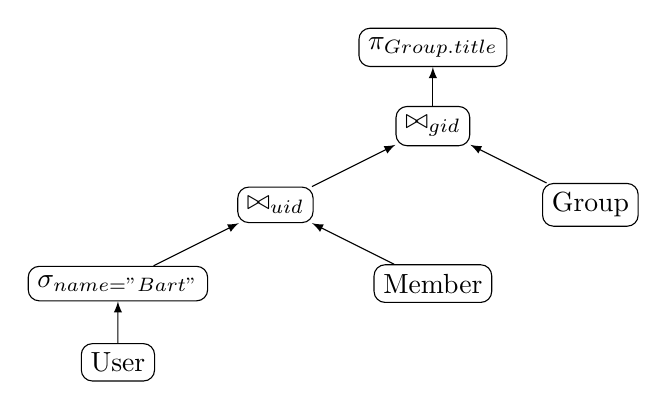
\begin{tikzpicture}[
            level distance=1.0cm,
            every node/.style={draw, rounded corners}, 
            sibling distance=4cm,
            edge from parent/.style={draw, latex-}  % Changed from -latex to latex-
        ]
        \node {$\pi_{\text{Group.title}}$}
            child {
                node {$\bowtie_{\text{gid}}$}
                child {
                    node {$\bowtie_{\text{uid}}$}
                    child {
                        node {$\sigma_{\text{name="Bart"}}$}
                        child {
                            node {User}
                        }
                    }
                    child {
                        node {Member}
                    }
                }
                child {
                    node {Group}
                }
            };
        \end{tikzpicture}
        \caption{Logical Plan. We first take User, select Bart, and join it to Member over uid. Then we join it with Group on gid, and finally project the title attribute.} 
        \label{fig:logical_plan}
      \end{figure}

      \begin{figure}[H]
        \centering 
        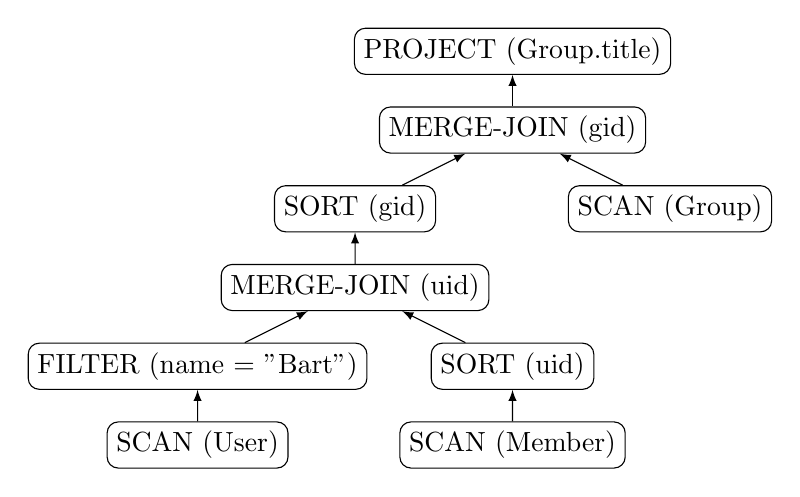
\begin{tikzpicture}[
            level distance=1.0cm,
            sibling distance=4cm,
            every node/.style={draw, rounded corners},
            edge from parent/.style={draw, latex-}  % Changed from -latex to latex-
        ]
        \node {PROJECT (Group.title)}
            child {
                node {MERGE-JOIN (gid)}
                child {
                    node {SORT (gid)}
                    child {
                        node {MERGE-JOIN (uid)}
                        child {
                            node {FILTER (name = "Bart")}
                            child {
                                node {SCAN (User)}
                            }
                        }
                        child {
                            node {SORT (uid)}
                            child {
                                node {SCAN (Member)}
                            }
                        }
                    }
                }
                child {
                    node {SCAN (Group)}
                }
            };
        \end{tikzpicture}
        \caption{Physical Plan. We first take User and do a scan before filtering/selecting tuples with Bart. We also scan Member and sort it by uid in order to prepare for merge-join. Once we merge-join over uid, we sort it again to prepare a second merge-join with Group (which we scan first). Once we do this, we finally project the title attribute. } 
        \label{fig:physical_plan}
      \end{figure}
    \end{example} 

  \subsubsection{SQL Rewrite}

    At the language level, SQL provides some APIs to force the DBMS to use a certain physical plan if desired. This requires expertise and should not be done by beginners, however. 

  \subsubsection{Cardinality Estimation}

    In the physical plan, we need to have a cost estimation for each operator. For example, we know that \texttt{SORT(gid)} takes $O(B(\text{input}) \cdot \log_M B(\text{input}))$, but we should find out what $B$, the number of blocks needed to store our input relation, is. To do this, we need the size of intermediate results through cardinality estimation.  

    Usually we cannot do quick and accurate cardinality estimation without strong assumptions, the first of which is uniformity of data. 

    \begin{example}[Selection with Equality Predicates]
      Suppose you have a relation $R$ with $|R| = 100,000$ tuples. Assume that it has an attribute $A$ taking integer values in $[50, 100)$ \textit{distributed uniformly}. Then, there are 50 distinct values, and when we want to do $\sigma_{A = a} (R)$, then we would expect it to return 
      \begin{equation}
        |\sigma_{A = a} (R)| = \frac{|R|}{|\pi_A(R)|} = 2000
      \end{equation}
      tuples.
    \end{example}

    The second assumption is \textit{independence} of the distributions over each attribute. 

    \begin{example}[Selection with Conjunctive Predicates]
      If we have the same relation $R$ with integer attributes $A \in [50, 100), B \in [10, 20)$ independently and uniformly distributed. Then, 
      \begin{equation}
        |\sigma_{A = a, B = b} (R) = \frac{|R|}{|\pi_A (R)| \cdot |\pi_B(R)|} = \frac{100,000}{50 \cdot 10} = 200
      \end{equation}
    \end{example}

    At this point, we are just using inclusion-exclusion principle and this becomes a counting problem. 

    \begin{example}[Negated, Disjunctive Predicates]
      We list these identities for brevity. The math is pretty simple. 
      \begin{equation}
        |\sigma_{A \neq a} (R)| = |R| \cdot \bigg( 1 - \frac{1}{|\pi_A (R)|} \bigg)
      \end{equation}
      and using I/E principle, we have 
      \begin{equation}
        |\sigma_{A = a \lor B = b} (R)| = |R| \cdot \bigg( \frac{1}{|\pi_A (R)|}  + \frac{1}{|\pi_B (R)|} - \frac{1}{|\pi_A (R)| \cdot |\pi_B(R)|} \bigg)
      \end{equation}
    \end{example}

    \begin{example}[Range Predicates]
      Range also works similarly, but only if we know the actual bounds of the attribute values.  
      \begin{equation}
        |\sigma_{A > a} (R)| = |R| \cdot \frac{\max(R.A) - a}{\max(R.A) - \min(R.A)}
      \end{equation}
    \end{example}

    Clearly, if we know that an attribute follows, say a Gaussian or a Poisson distribution, we can just calculate the difference in the CDFs and scale up by the relation size to get the approximate cardinality. I think this is what the professor refers to as \textit{histogram estimation}. 

    For joins, we need yet another assumption, called \textit{containment of value sets}. This means that if we are natural joining $R(A, B) \bowtie S(A, C)$, every tuple in the smaller (as in fewer distinct values for the join attribute $A$) joins with some tuple in the other relation. In other words, 
    \begin{equation}
      |\pi_A (R)| \leq |\pi_A (S)| \implies \pi_A (R) \subset \pi_A (S)
    \end{equation}
    which again is a very strong assumption in general but holds in the case of foreign key joins. 

    \begin{example}[Two Way Equi-Join] 
      With the containment assumption, we have 
      \begin{equation}
        |R \bowtie_{A} S| = \frac{|R| \cdot |S|}{\max( |\pi_A (R)|, |\pi_A(S)|)}
      \end{equation} 
      Think of this as looking at the cross product between the two relations, and then filtering out the actual tuples that don't belong there.  
    \end{example}

\subsection{Exercises} 

  Let's do a more comprehensive exercise. 

  \begin{example}[Cost Estimation of Physical Query Plan]
    Say we have three relations 
    \begin{enumerate}
      \item \texttt{Student(\underline{sid}, name, age, addr)}. $T(S) = 10,000$ tuples, $B(S) = 1,000$ pages. 
      \item \texttt{Book(\underline{bid}, title, author)}. $T(B) = 50,000$ tuples, $B(S) = 5,000$ pages. 
      \item \texttt{Checkout(\underline{sid}, \underline{bid}, date)}. $T(C) = 300,000$ tuples, $B(C) = 15,000$ pages. 
    \end{enumerate}
    And say that the number of \texttt{author} attribute values in \texttt{Book} with $7 \leq \texttt{age} \leq 24$ is 500 tuples. There is an unclustered B+ tree index on \texttt{B.author}, a clustered B+ tree index on \texttt{C.bid}, and all index pages are in memory. Also we assume unlimited memory to simplify things. 
    \begin{figure}[H]
      \centering 
      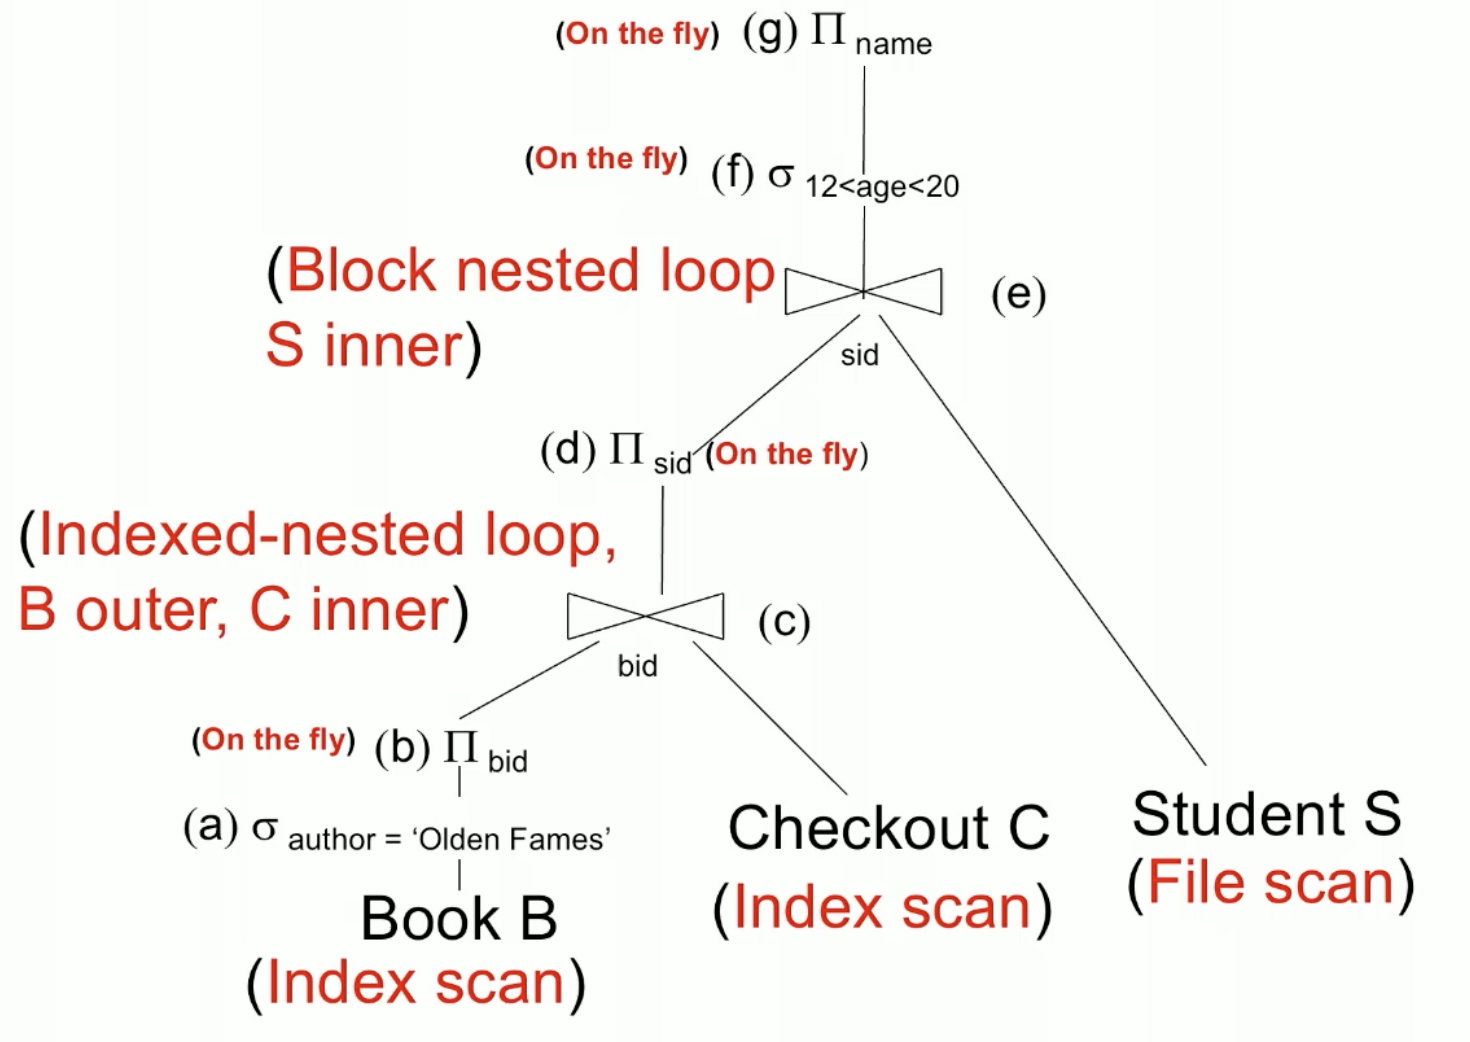
\includegraphics[scale=0.4]{img/book_plan.png}
      \caption{We have the following physical plan.} 
      \label{fig:book_plan}
    \end{figure} 
    Okay, so let's do this. Note that since all index pages are in memory, we are storing the entire B+ tree in memory and don't need extra IOs to traverse it.  
    \begin{enumerate}
      \item[a)] For the selection, the author is an unclustered B+ tree. There are 50,000 tuples and 500 distinct authors. Since we're querying 1 author, by uniformity we would need to access $100$ book which may all be in their own disk page, so we need $100$ IOs.\footnote{If this was clustered, then each page can store $10$ tuples, so we actually need $10$ IOs. } We end up with an output relation of 100 tuples in memory, so we also have a cardinality of $100$. 
        \begin{equation}
          \mathrm{IO}(a) = \frac{T(B)}{500} = \frac{50,000}{500} = 100, \; \mathrm{Card}(a) = 100 
        \end{equation}

      \item[b)] For the projection on \texttt{bid}, we have already loaded in our relation in memory, so the IO cost is $0$. We are still working with 100 pages, so our cardinality is still $100$. 
        \begin{equation}
          \mathrm{IO} = 0, \; \mathrm{Card}(b) = 100 
        \end{equation} 

      \item[c)] Now we do a join with an index-nested loop join on \texttt{bid}. Recall that we want to use the value of the outer table \texttt{R.bid} to probe the index on the inner table \texttt{C.bid}, which is clustered. We already have our outer table in memory, and we use the index \texttt{bid} to probe our inner table \texttt{C}. For each of the 50,000 book tuples in \texttt{B}, there are 300,000 checkout tuples in \texttt{C}, meaning that there are about $300,000/50,000 = 6$ checkout per book. For each of the 100 book tuples in (a), we expect to get 6 checkouts per book. There are $300,000 / 15,000 = 20$ checkout tuples per page, so counting for page boundaries we assume that 6 tuples will fit in at most 2 pages (or maybe 1). Therefore, we have 
        \begin{equation}
          \mathrm{IO}(c) = 100 \cdot 2 = 200, \; \mathrm{Card}(c) = 100 \cdot 6 = 600
        \end{equation}

      \item[d)] This is done in memory so IO is $0$. Note that we have a total of 600 checkout/book tuples. Since this is a projection, the cardinality also remains the same. 
        \begin{equation}
          \mathrm{IO}(d) = 0, \; \mathrm{Card}(d) = 600 
        \end{equation}

      \item[e)] Now we have a block nested loop join. Since (d) is already in memory (on the fly), all we have to do is load all of \texttt{S} into memory (unlimited), which means our IO cost is $B(S) = 1000$. We are joining with the student relation, and since there is 1 student per checkout, our output relation is still 600 tuples long. 
        \begin{equation}
          \mathrm{IO}(e) = 1000, \; \mathrm{Card}(e) = 600
        \end{equation}

      \item[f)] Finally we select, and assuming that the ages are uniformly distributed, we expect $(20 - 12 - 1)/ (24 - 7 + 1) = 7/18$ of the relations to remain after selection. IO is $0$ since this is on the fly. 
        \begin{equation}
          \mathrm{IO}(f) = 0, \; \mathrm{Card}(f) = 600 \cdot \frac{7}{18} \approx 234
        \end{equation}

      \item[g)] Finally, we project onto name. IO is $0$ since on the fly. We are projecting on names and assuming we don't remove duplicates\footnote{Is this really a realistic assumption?} our output relation is still the same length. 
        \begin{equation}
          \mathrm{IO}(g) = 0, \; \mathrm{Card}(g) = 234
        \end{equation}
    \end{enumerate}
    The total cost is $1000 + 200 + 100 = 1300$ and the final cardinality is $234$. 
  \end{example}

